\documentclass[1p]{elsarticle_modified}
%\bibliographystyle{elsarticle-num}

%\usepackage[colorlinks]{hyperref}
%\usepackage{abbrmath_seonhwa} %\Abb, \Ascr, \Acal ,\Abf, \Afrak
\usepackage{amsfonts}
\usepackage{amssymb}
\usepackage{amsmath}
\usepackage{amsthm}
\usepackage{scalefnt}
\usepackage{amsbsy}
\usepackage{kotex}
\usepackage{caption}
\usepackage{subfig}
\usepackage{color}
\usepackage{graphicx}
\usepackage{xcolor} %% white, black, red, green, blue, cyan, magenta, yellow
\usepackage{float}
\usepackage{setspace}
\usepackage{hyperref}

\usepackage{tikz}
\usetikzlibrary{arrows}

\usepackage{multirow}
\usepackage{array} % fixed length table
\usepackage{hhline}

%%%%%%%%%%%%%%%%%%%%%
\makeatletter
\renewcommand*\env@matrix[1][\arraystretch]{%
	\edef\arraystretch{#1}%
	\hskip -\arraycolsep
	\let\@ifnextchar\new@ifnextchar
	\array{*\c@MaxMatrixCols c}}
\makeatother %https://tex.stackexchange.com/questions/14071/how-can-i-increase-the-line-spacing-in-a-matrix
%%%%%%%%%%%%%%%

\usepackage[normalem]{ulem}

\newcommand{\msout}[1]{\ifmmode\text{\sout{\ensuremath{#1}}}\else\sout{#1}\fi}
%SOURCE: \msout is \stkout macro in https://tex.stackexchange.com/questions/20609/strikeout-in-math-mode

\newcommand{\cancel}[1]{
	\ifmmode
	{\color{red}\msout{#1}}
	\else
	{\color{red}\sout{#1}}
	\fi
}

\newcommand{\add}[1]{
	{\color{blue}\uwave{#1}}
}

\newcommand{\replace}[2]{
	\ifmmode
	{\color{red}\msout{#1}}{\color{blue}\uwave{#2}}
	\else
	{\color{red}\sout{#1}}{\color{blue}\uwave{#2}}
	\fi
}

\newcommand{\Sol}{\mathcal{S}} %segment
\newcommand{\D}{D} %diagram
\newcommand{\A}{\mathcal{A}} %arc


%%%%%%%%%%%%%%%%%%%%%%%%%%%%%5 test

\def\sl{\operatorname{\textup{SL}}(2,\Cbb)}
\def\psl{\operatorname{\textup{PSL}}(2,\Cbb)}
\def\quan{\mkern 1mu \triangleright \mkern 1mu}

\theoremstyle{definition}
\newtheorem{thm}{Theorem}[section]
\newtheorem{prop}[thm]{Proposition}
\newtheorem{lem}[thm]{Lemma}
\newtheorem{ques}[thm]{Question}
\newtheorem{cor}[thm]{Corollary}
\newtheorem{defn}[thm]{Definition}
\newtheorem{exam}[thm]{Example}
\newtheorem{rmk}[thm]{Remark}
\newtheorem{alg}[thm]{Algorithm}

\newcommand{\I}{\sqrt{-1}}
\begin{document}

%\begin{frontmatter}
%
%\title{Boundary parabolic representations of knots up to 8 crossings}
%
%%% Group authors per affiliation:
%\author{Yunhi Cho} 
%\address{Department of Mathematics, University of Seoul, Seoul, Korea}
%\ead{yhcho@uos.ac.kr}
%
%
%\author{Seonhwa Kim} %\fnref{s_kim}}
%\address{Center for Geometry and Physics, Institute for Basic Science, Pohang, 37673, Korea}
%\ead{ryeona17@ibs.re.kr}
%
%\author{Hyuk Kim}
%\address{Department of Mathematical Sciences, Seoul National University, Seoul 08826, Korea}
%\ead{hyukkim@snu.ac.kr}
%
%\author{Seokbeom Yoon}
%\address{Department of Mathematical Sciences, Seoul National University, Seoul, 08826,  Korea}
%\ead{sbyoon15@snu.ac.kr}
%
%\begin{abstract}
%We find all boundary parabolic representation of knots up to 8 crossings.
%
%\end{abstract}
%\begin{keyword}
%    \MSC[2010] 57M25 
%\end{keyword}
%
%\end{frontmatter}

%\linenumbers
%\tableofcontents
%
\newcommand\colored[1]{\textcolor{white}{\rule[-0.35ex]{0.8em}{1.4ex}}\kern-0.8em\color{red} #1}%
%\newcommand\colored[1]{\textcolor{white}{ #1}\kern-2.17ex	\textcolor{white}{ #1}\kern-1.81ex	\textcolor{white}{ #1}\kern-2.15ex\color{red}#1	}

{\Large $\underline{12a_{1268}~(K12a_{1268})}$}

\setlength{\tabcolsep}{10pt}
\renewcommand{\arraystretch}{1.6}
\vspace{1cm}\begin{tabular}{m{100pt}>{\centering\arraybackslash}m{274pt}}
\multirow{5}{120pt}{
	\centering
	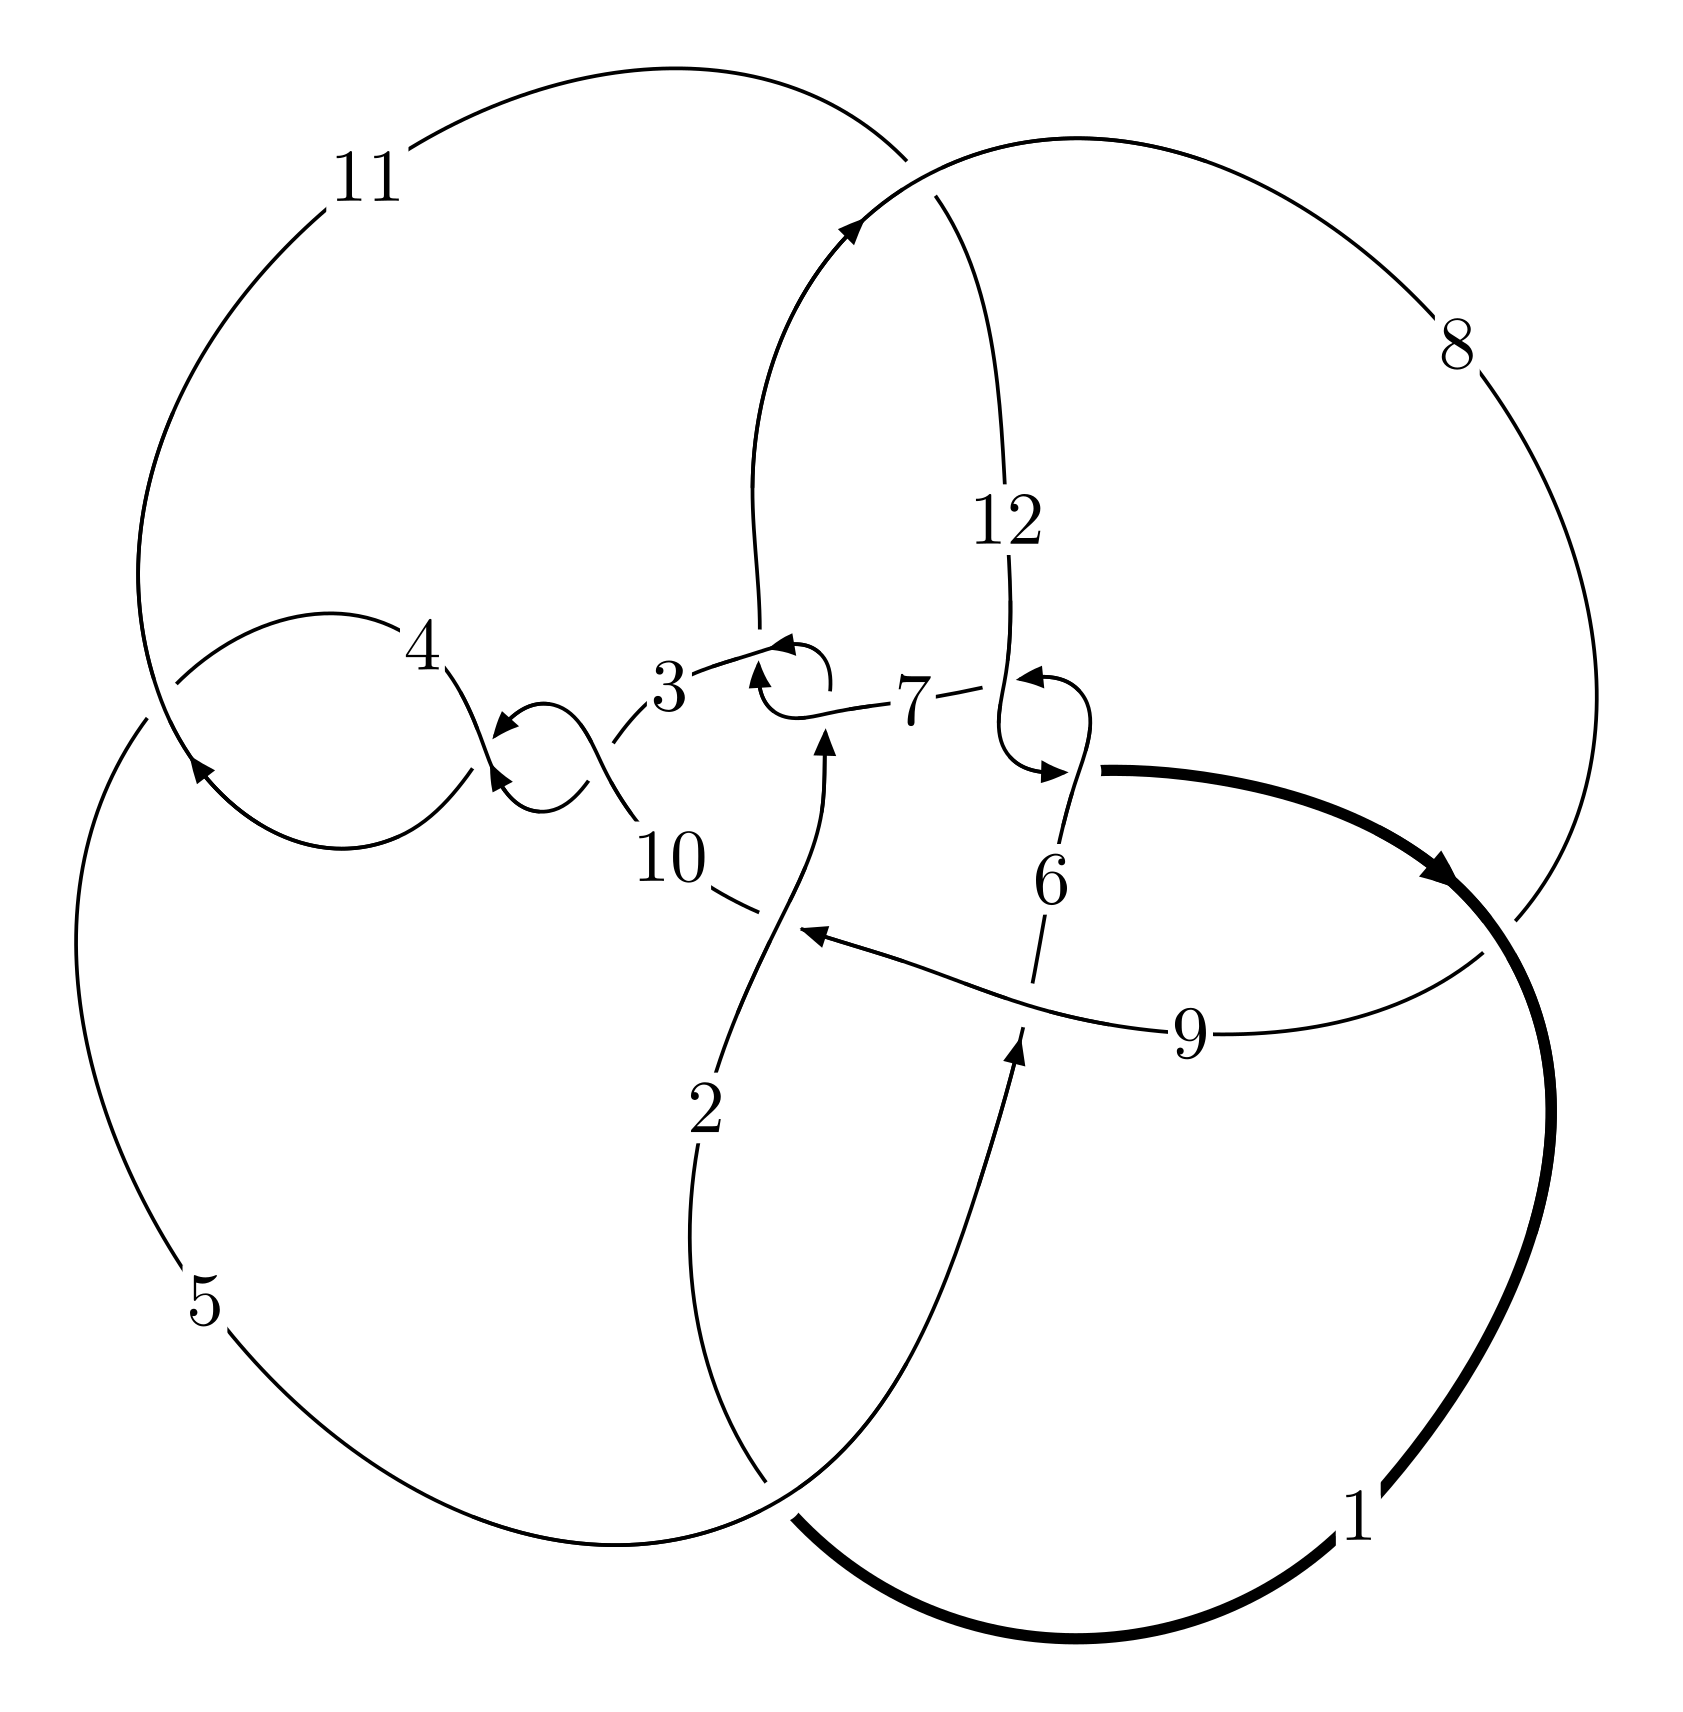
\includegraphics[width=112pt]{../../../GIT/diagram.site/Diagrams/png/2069_12a_1268.png}\\
\ \ \ A knot diagram\footnotemark}&
\allowdisplaybreaks
\textbf{Linearized knot diagam} \\
\cline{2-2}
 &
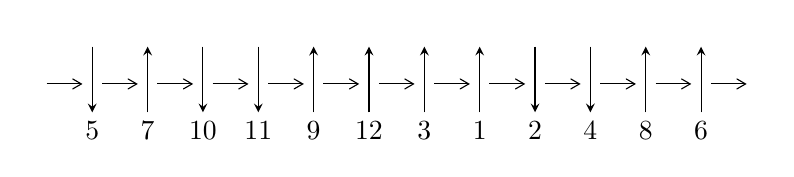
\begin{tikzpicture}[x=20pt, y=17pt]
	% nodes
	\node (C0) at (0, 0) {};
	\node (C1) at (1, 0) {};
	\node (C1U) at (1, +1) {};
	\node (C1D) at (1, -1) {5};

	\node (C2) at (2, 0) {};
	\node (C2U) at (2, +1) {};
	\node (C2D) at (2, -1) {7};

	\node (C3) at (3, 0) {};
	\node (C3U) at (3, +1) {};
	\node (C3D) at (3, -1) {10};

	\node (C4) at (4, 0) {};
	\node (C4U) at (4, +1) {};
	\node (C4D) at (4, -1) {11};

	\node (C5) at (5, 0) {};
	\node (C5U) at (5, +1) {};
	\node (C5D) at (5, -1) {9};

	\node (C6) at (6, 0) {};
	\node (C6U) at (6, +1) {};
	\node (C6D) at (6, -1) {12};

	\node (C7) at (7, 0) {};
	\node (C7U) at (7, +1) {};
	\node (C7D) at (7, -1) {3};

	\node (C8) at (8, 0) {};
	\node (C8U) at (8, +1) {};
	\node (C8D) at (8, -1) {1};

	\node (C9) at (9, 0) {};
	\node (C9U) at (9, +1) {};
	\node (C9D) at (9, -1) {2};

	\node (C10) at (10, 0) {};
	\node (C10U) at (10, +1) {};
	\node (C10D) at (10, -1) {4};

	\node (C11) at (11, 0) {};
	\node (C11U) at (11, +1) {};
	\node (C11D) at (11, -1) {8};

	\node (C12) at (12, 0) {};
	\node (C12U) at (12, +1) {};
	\node (C12D) at (12, -1) {6};
	\node (C13) at (13, 0) {};

	% arrows
	\draw[->,>={angle 60}]
	(C0) edge (C1) (C1) edge (C2) (C2) edge (C3) (C3) edge (C4) (C4) edge (C5) (C5) edge (C6) (C6) edge (C7) (C7) edge (C8) (C8) edge (C9) (C9) edge (C10) (C10) edge (C11) (C11) edge (C12) (C12) edge (C13) ;	\draw[->,>=stealth]
	(C1U) edge (C1D) (C2D) edge (C2U) (C3U) edge (C3D) (C4U) edge (C4D) (C5D) edge (C5U) (C6D) edge (C6U) (C7D) edge (C7U) (C8D) edge (C8U) (C9U) edge (C9D) (C10U) edge (C10D) (C11D) edge (C11U) (C12D) edge (C12U) ;
	\end{tikzpicture} \\
\hhline{~~} \\& 
\textbf{Solving Sequence} \\ \cline{2-2} 
 &
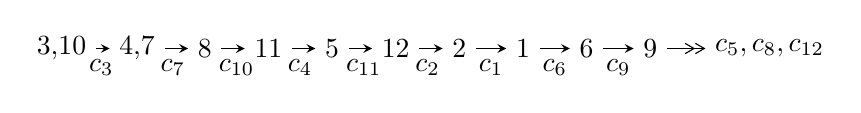
\begin{tikzpicture}[x=23pt, y=7pt]
	% node
	\node (A0) at (-1/8, 0) {3,10};
	\node (A1) at (17/16, 0) {4,7};
	\node (A2) at (17/8, 0) {8};
	\node (A3) at (25/8, 0) {11};
	\node (A4) at (33/8, 0) {5};
	\node (A5) at (41/8, 0) {12};
	\node (A6) at (49/8, 0) {2};
	\node (A7) at (57/8, 0) {1};
	\node (A8) at (65/8, 0) {6};
	\node (A9) at (73/8, 0) {9};
	\node (C1) at (1/2, -1) {$c_{3}$};
	\node (C2) at (13/8, -1) {$c_{7}$};
	\node (C3) at (21/8, -1) {$c_{10}$};
	\node (C4) at (29/8, -1) {$c_{4}$};
	\node (C5) at (37/8, -1) {$c_{11}$};
	\node (C6) at (45/8, -1) {$c_{2}$};
	\node (C7) at (53/8, -1) {$c_{1}$};
	\node (C8) at (61/8, -1) {$c_{6}$};
	\node (C9) at (69/8, -1) {$c_{9}$};
	\node (A10) at (11, 0) {$c_{5},c_{8},c_{12}$};

	% edge
	\draw[->,>=stealth]	
	(A0) edge (A1) (A1) edge (A2) (A2) edge (A3) (A3) edge (A4) (A4) edge (A5) (A5) edge (A6) (A6) edge (A7) (A7) edge (A8) (A8) edge (A9) ;
	\draw[->>,>={angle 60}]	
	(A9) edge (A10);
\end{tikzpicture} \\ 

\end{tabular} \\

\footnotetext{
The image of knot diagram is generated by the software ``\textbf{Draw programme}" developed by Andrew Bartholomew(\url{http://www.layer8.co.uk/maths/draw/index.htm\#Running-draw}), where we modified some parts for our purpose(\url{https://github.com/CATsTAILs/LinksPainter}).
}\phantom \\ \newline 
\centering \textbf{Ideals for irreducible components\footnotemark of $X_{\text{par}}$} 
 
\begin{align*}
I^u_{1}&=\langle 
9.11346\times10^{461} u^{147}+3.95273\times10^{461} u^{146}+\cdots+3.62863\times10^{462} b-1.72199\times10^{463},\\
\phantom{I^u_{1}}&\phantom{= \langle  }4.51564\times10^{464} u^{147}+9.26536\times10^{463} u^{146}+\cdots+1.34259\times10^{464} a-2.14693\times10^{466},\\
\phantom{I^u_{1}}&\phantom{= \langle  }u^{148}- u^{147}+\cdots-565 u+37\rangle \\
I^u_{2}&=\langle 
-21787693 u^{37}-17833328 u^{36}+\cdots+4484003 b+11235058,\\
\phantom{I^u_{2}}&\phantom{= \langle  }4256822446 u^{37}+1213250697 u^{36}+\cdots+587404393 a-4089312198,\;u^{38}-20 u^{36}+\cdots-2 u+1\rangle \\
\\
\end{align*}
\raggedright * 2 irreducible components of $\dim_{\mathbb{C}}=0$, with total 186 representations.\\
\footnotetext{All coefficients of polynomials are rational numbers. But the coefficients are sometimes approximated in decimal forms when there is not enough margin.}
\newpage
\renewcommand{\arraystretch}{1}
\centering \section*{I. $I^u_{1}= \langle 9.11\times10^{461} u^{147}+3.95\times10^{461} u^{146}+\cdots+3.63\times10^{462} b-1.72\times10^{463},\;4.52\times10^{464} u^{147}+9.27\times10^{463} u^{146}+\cdots+1.34\times10^{464} a-2.15\times10^{466},\;u^{148}- u^{147}+\cdots-565 u+37 \rangle$}
\flushleft \textbf{(i) Arc colorings}\\
\begin{tabular}{m{7pt} m{180pt} m{7pt} m{180pt} }
\flushright $a_{3}=$&$\begin{pmatrix}1\\0\end{pmatrix}$ \\
\flushright $a_{10}=$&$\begin{pmatrix}0\\u\end{pmatrix}$ \\
\flushright $a_{4}=$&$\begin{pmatrix}1\\u^2\end{pmatrix}$ \\
\flushright $a_{7}=$&$\begin{pmatrix}-3.36337 u^{147}-0.690109 u^{146}+\cdots-1732.60 u+159.909\\-0.251154 u^{147}-0.108932 u^{146}+\cdots-88.7224 u+4.74555\end{pmatrix}$ \\
\flushright $a_{8}=$&$\begin{pmatrix}-3.61452 u^{147}-0.799040 u^{146}+\cdots-1821.32 u+164.655\\-0.251154 u^{147}-0.108932 u^{146}+\cdots-88.7224 u+4.74555\end{pmatrix}$ \\
\flushright $a_{11}=$&$\begin{pmatrix}- u\\- u^3+u\end{pmatrix}$ \\
\flushright $a_{5}=$&$\begin{pmatrix}- u^2+1\\- u^4+2 u^2\end{pmatrix}$ \\
\flushright $a_{12}=$&$\begin{pmatrix}-0.585914 u^{147}+0.232383 u^{146}+\cdots-797.840 u+110.149\\1.37060 u^{147}+0.380173 u^{146}+\cdots+566.237 u-37.5510\end{pmatrix}$ \\
\flushright $a_{2}=$&$\begin{pmatrix}-1.84258 u^{147}-0.465549 u^{146}+\cdots-904.057 u+86.1561\\-0.299998 u^{147}-0.0844511 u^{146}+\cdots-89.1876 u+3.14636\end{pmatrix}$ \\
\flushright $a_{1}=$&$\begin{pmatrix}-2.61434 u^{147}-0.697404 u^{146}+\cdots-1189.37 u+102.524\\0.372888 u^{147}+0.126054 u^{146}+\cdots+198.348 u-16.7759\end{pmatrix}$ \\
\flushright $a_{6}=$&$\begin{pmatrix}4.65490 u^{147}+1.63243 u^{146}+\cdots+1539.37 u-78.1800\\-0.150348 u^{147}-0.0242958 u^{146}+\cdots-118.307 u+13.7502\end{pmatrix}$ \\
\flushright $a_{9}=$&$\begin{pmatrix}-1.51255 u^{147}-0.235174 u^{146}+\cdots-911.852 u+102.320\\-0.818133 u^{147}-0.239079 u^{146}+\cdots-290.745 u+17.0314\end{pmatrix}$\\&\end{tabular}
\flushleft \textbf{(ii) Obstruction class $= -1$}\\~\\
\flushleft \textbf{(iii) Cusp Shapes $= -0.568977 u^{147}+0.0557856 u^{146}+\cdots-394.985 u+37.7750$}\\~\\
\newpage\renewcommand{\arraystretch}{1}
\flushleft \textbf{(iv) u-Polynomials at the component}\newline \\
\begin{tabular}{m{50pt}|m{274pt}}
Crossings & \hspace{64pt}u-Polynomials at each crossing \\
\hline $$\begin{aligned}c_{1}\end{aligned}$$&$\begin{aligned}
&u^{148}+5 u^{147}+\cdots-47 u+1
\end{aligned}$\\
\hline $$\begin{aligned}c_{2},c_{7}\end{aligned}$$&$\begin{aligned}
&u^{148}+u^{147}+\cdots+28032 u+9472
\end{aligned}$\\
\hline $$\begin{aligned}c_{3},c_{4},c_{10}\end{aligned}$$&$\begin{aligned}
&u^{148}+u^{147}+\cdots+565 u+37
\end{aligned}$\\
\hline $$\begin{aligned}c_{5}\end{aligned}$$&$\begin{aligned}
&u^{148}-5 u^{147}+\cdots+207817 u+10777
\end{aligned}$\\
\hline $$\begin{aligned}c_{6},c_{12}\end{aligned}$$&$\begin{aligned}
&u^{148}+u^{147}+\cdots-4721 u+6513
\end{aligned}$\\
\hline $$\begin{aligned}c_{8}\end{aligned}$$&$\begin{aligned}
&u^{148}+15 u^{146}+\cdots+608 u+64
\end{aligned}$\\
\hline $$\begin{aligned}c_{9}\end{aligned}$$&$\begin{aligned}
&u^{148}-3 u^{147}+\cdots+733241455 u+110567423
\end{aligned}$\\
\hline $$\begin{aligned}c_{11}\end{aligned}$$&$\begin{aligned}
&u^{148}+u^{147}+\cdots-13110 u+65501
\end{aligned}$\\
\hline
\end{tabular}\\~\\
\newpage\renewcommand{\arraystretch}{1}
\flushleft \textbf{(v) Riley Polynomials at the component}\newline \\
\begin{tabular}{m{50pt}|m{274pt}}
Crossings & \hspace{64pt}Riley Polynomials at each crossing \\
\hline $$\begin{aligned}c_{1}\end{aligned}$$&$\begin{aligned}
&y^{148}+7 y^{147}+\cdots-253 y+1
\end{aligned}$\\
\hline $$\begin{aligned}c_{2},c_{7}\end{aligned}$$&$\begin{aligned}
&y^{148}-71 y^{147}+\cdots-3723476992 y+89718784
\end{aligned}$\\
\hline $$\begin{aligned}c_{3},c_{4},c_{10}\end{aligned}$$&$\begin{aligned}
&y^{148}-143 y^{147}+\cdots-187357 y+1369
\end{aligned}$\\
\hline $$\begin{aligned}c_{5}\end{aligned}$$&$\begin{aligned}
&y^{148}+35 y^{147}+\cdots-9055314399 y+116143729
\end{aligned}$\\
\hline $$\begin{aligned}c_{6},c_{12}\end{aligned}$$&$\begin{aligned}
&y^{148}+111 y^{147}+\cdots+1135280675 y+42419169
\end{aligned}$\\
\hline $$\begin{aligned}c_{8}\end{aligned}$$&$\begin{aligned}
&y^{148}+30 y^{147}+\cdots+113664 y+4096
\end{aligned}$\\
\hline $$\begin{aligned}c_{9}\end{aligned}$$&$\begin{aligned}
&y^{148}-27 y^{147}+\cdots-884023777418158187 y+12225155028860929
\end{aligned}$\\
\hline $$\begin{aligned}c_{11}\end{aligned}$$&$\begin{aligned}
&y^{148}+21 y^{147}+\cdots+171350880528 y+4290381001
\end{aligned}$\\
\hline
\end{tabular}\\~\\
\newpage\flushleft \textbf{(vi) Complex Volumes and Cusp Shapes}
$$\begin{array}{c|c|c}  
\text{Solutions to }I^u_{1}& \I (\text{vol} + \sqrt{-1}CS) & \text{Cusp shape}\\
 \hline 
\begin{aligned}
u &= \phantom{-}0.231974 + 0.965550 I \\
a &= \phantom{-}1.61605 + 0.24726 I \\
b &= -0.942533 + 0.407635 I\end{aligned}
 & \phantom{-}2.28070 - 2.18616 I & \phantom{-0.000000 } 0 \\ \hline\begin{aligned}
u &= \phantom{-}0.231974 - 0.965550 I \\
a &= \phantom{-}1.61605 - 0.24726 I \\
b &= -0.942533 - 0.407635 I\end{aligned}
 & \phantom{-}2.28070 + 2.18616 I & \phantom{-0.000000 } 0 \\ \hline\begin{aligned}
u &= \phantom{-}0.357273 + 0.925002 I \\
a &= -1.82625 - 0.10771 I \\
b &= \phantom{-}1.147880 - 0.497498 I\end{aligned}
 & \phantom{-}3.40517 - 8.71558 I & \phantom{-0.000000 } 0 \\ \hline\begin{aligned}
u &= \phantom{-}0.357273 - 0.925002 I \\
a &= -1.82625 + 0.10771 I \\
b &= \phantom{-}1.147880 + 0.497498 I\end{aligned}
 & \phantom{-}3.40517 + 8.71558 I & \phantom{-0.000000 } 0 \\ \hline\begin{aligned}
u &= \phantom{-}0.498173 + 0.850756 I \\
a &= \phantom{-}0.924558 + 0.879436 I \\
b &= -0.899190 - 0.367524 I\end{aligned}
 & -1.79766 + 2.02965 I & \phantom{-0.000000 } 0 \\ \hline\begin{aligned}
u &= \phantom{-}0.498173 - 0.850756 I \\
a &= \phantom{-}0.924558 - 0.879436 I \\
b &= -0.899190 + 0.367524 I\end{aligned}
 & -1.79766 - 2.02965 I & \phantom{-0.000000 } 0 \\ \hline\begin{aligned}
u &= -0.403377 + 0.895392 I \\
a &= \phantom{-}1.87705 - 0.26722 I \\
b &= -1.203460 - 0.645179 I\end{aligned}
 & -1.2856 + 14.9681 I & \phantom{-0.000000 } 0 \\ \hline\begin{aligned}
u &= -0.403377 - 0.895392 I \\
a &= \phantom{-}1.87705 + 0.26722 I \\
b &= -1.203460 + 0.645179 I\end{aligned}
 & -1.2856 - 14.9681 I & \phantom{-0.000000 } 0 \\ \hline\begin{aligned}
u &= -0.581403 + 0.840266 I \\
a &= -1.58415 + 0.76045 I \\
b &= \phantom{-}1.077340 + 0.458818 I\end{aligned}
 & \phantom{-}1.49467 + 5.83890 I & \phantom{-0.000000 } 0 \\ \hline\begin{aligned}
u &= -0.581403 - 0.840266 I \\
a &= -1.58415 - 0.76045 I \\
b &= \phantom{-}1.077340 - 0.458818 I\end{aligned}
 & \phantom{-}1.49467 - 5.83890 I & \phantom{-0.000000 } 0\\
 \hline 
 \end{array}$$\newpage$$\begin{array}{c|c|c}  
\text{Solutions to }I^u_{1}& \I (\text{vol} + \sqrt{-1}CS) & \text{Cusp shape}\\
 \hline 
\begin{aligned}
u &= -0.919473 + 0.484488 I \\
a &= \phantom{-}0.0697847 - 0.0236496 I \\
b &= -0.961453 + 0.453445 I\end{aligned}
 & -1.63528 + 2.03359 I & \phantom{-0.000000 } 0 \\ \hline\begin{aligned}
u &= -0.919473 - 0.484488 I \\
a &= \phantom{-}0.0697847 + 0.0236496 I \\
b &= -0.961453 - 0.453445 I\end{aligned}
 & -1.63528 - 2.03359 I & \phantom{-0.000000 } 0 \\ \hline\begin{aligned}
u &= -0.439196 + 0.782732 I \\
a &= \phantom{-}1.55816 - 0.07528 I \\
b &= -0.865042 - 0.251362 I\end{aligned}
 & \phantom{-}1.171650 - 0.269264 I & \phantom{-0.000000 } 0 \\ \hline\begin{aligned}
u &= -0.439196 - 0.782732 I \\
a &= \phantom{-}1.55816 + 0.07528 I \\
b &= -0.865042 + 0.251362 I\end{aligned}
 & \phantom{-}1.171650 + 0.269264 I & \phantom{-0.000000 } 0 \\ \hline\begin{aligned}
u &= -0.826059 + 0.740595 I \\
a &= -0.814168 + 0.620310 I \\
b &= \phantom{-}1.072910 - 0.550619 I\end{aligned}
 & -2.53181 - 9.42226 I & \phantom{-0.000000 } 0 \\ \hline\begin{aligned}
u &= -0.826059 - 0.740595 I \\
a &= -0.814168 - 0.620310 I \\
b &= \phantom{-}1.072910 + 0.550619 I\end{aligned}
 & -2.53181 + 9.42226 I & \phantom{-0.000000 } 0 \\ \hline\begin{aligned}
u &= -0.034444 + 0.878485 I \\
a &= \phantom{-}1.89031 + 0.70285 I \\
b &= -0.860373 - 0.345168 I\end{aligned}
 & -1.96259 + 1.02583 I & \phantom{-0.000000 } 0 \\ \hline\begin{aligned}
u &= -0.034444 - 0.878485 I \\
a &= \phantom{-}1.89031 - 0.70285 I \\
b &= -0.860373 + 0.345168 I\end{aligned}
 & -1.96259 - 1.02583 I & \phantom{-0.000000 } 0 \\ \hline\begin{aligned}
u &= \phantom{-}0.534463 + 0.676615 I \\
a &= -1.50415 - 0.26281 I \\
b &= \phantom{-}1.141460 - 0.585695 I\end{aligned}
 & -2.15552 - 6.96261 I & \phantom{-0.000000 } 0 \\ \hline\begin{aligned}
u &= \phantom{-}0.534463 - 0.676615 I \\
a &= -1.50415 + 0.26281 I \\
b &= \phantom{-}1.141460 + 0.585695 I\end{aligned}
 & -2.15552 + 6.96261 I & \phantom{-0.000000 } 0\\
 \hline 
 \end{array}$$\newpage$$\begin{array}{c|c|c}  
\text{Solutions to }I^u_{1}& \I (\text{vol} + \sqrt{-1}CS) & \text{Cusp shape}\\
 \hline 
\begin{aligned}
u &= -1.134210 + 0.178307 I \\
a &= \phantom{-}0.377680 - 1.136420 I \\
b &= -1.174710 - 0.194516 I\end{aligned}
 & -0.73408 - 2.34311 I & \phantom{-0.000000 } 0 \\ \hline\begin{aligned}
u &= -1.134210 - 0.178307 I \\
a &= \phantom{-}0.377680 + 1.136420 I \\
b &= -1.174710 + 0.194516 I\end{aligned}
 & -0.73408 + 2.34311 I & \phantom{-0.000000 } 0 \\ \hline\begin{aligned}
u &= -0.085848 + 0.829903 I \\
a &= -1.269460 + 0.287223 I \\
b &= \phantom{-}0.925969 + 0.640871 I\end{aligned}
 & \phantom{-}1.02925 + 2.54980 I & \phantom{-0.000000 } 0 \\ \hline\begin{aligned}
u &= -0.085848 - 0.829903 I \\
a &= -1.269460 - 0.287223 I \\
b &= \phantom{-}0.925969 - 0.640871 I\end{aligned}
 & \phantom{-}1.02925 - 2.54980 I & \phantom{-0.000000 } 0 \\ \hline\begin{aligned}
u &= -0.559642 + 0.607958 I \\
a &= \phantom{-}1.235330 - 0.392564 I \\
b &= -0.883726 + 0.285594 I\end{aligned}
 & \phantom{-}1.61185 - 0.79071 I & \phantom{-0.000000 } 0 \\ \hline\begin{aligned}
u &= -0.559642 - 0.607958 I \\
a &= \phantom{-}1.235330 + 0.392564 I \\
b &= -0.883726 - 0.285594 I\end{aligned}
 & \phantom{-}1.61185 + 0.79071 I & \phantom{-0.000000 } 0 \\ \hline\begin{aligned}
u &= -1.18648\phantom{ +0.000000I} \\
a &= \phantom{-}1.47562\phantom{ +0.000000I} \\
b &= -1.37704\phantom{ +0.000000I}\end{aligned}
 & \phantom{-}2.50742\phantom{ +0.000000I} & \phantom{-0.000000 } 0 \\ \hline\begin{aligned}
u &= \phantom{-}0.406779 + 0.689175 I \\
a &= \phantom{-}0.313889 + 0.646488 I \\
b &= -0.341716 - 1.020640 I\end{aligned}
 & -3.95306 - 9.00700 I & \phantom{-0.000000 } 0 \\ \hline\begin{aligned}
u &= \phantom{-}0.406779 - 0.689175 I \\
a &= \phantom{-}0.313889 - 0.646488 I \\
b &= -0.341716 + 1.020640 I\end{aligned}
 & -3.95306 + 9.00700 I & \phantom{-0.000000 } 0 \\ \hline\begin{aligned}
u &= \phantom{-}1.170200 + 0.268964 I \\
a &= -0.669958 - 0.078471 I \\
b &= \phantom{-}1.139010 + 0.011760 I\end{aligned}
 & -1.83354 - 2.63838 I & \phantom{-0.000000 } 0\\
 \hline 
 \end{array}$$\newpage$$\begin{array}{c|c|c}  
\text{Solutions to }I^u_{1}& \I (\text{vol} + \sqrt{-1}CS) & \text{Cusp shape}\\
 \hline 
\begin{aligned}
u &= \phantom{-}1.170200 - 0.268964 I \\
a &= -0.669958 + 0.078471 I \\
b &= \phantom{-}1.139010 - 0.011760 I\end{aligned}
 & -1.83354 + 2.63838 I & \phantom{-0.000000 } 0 \\ \hline\begin{aligned}
u &= -1.202940 + 0.056948 I \\
a &= \phantom{-}0.49506 - 1.40003 I \\
b &= -0.916918 - 0.221604 I\end{aligned}
 & -0.57689 - 2.41463 I & \phantom{-0.000000 } 0 \\ \hline\begin{aligned}
u &= -1.202940 - 0.056948 I \\
a &= \phantom{-}0.49506 + 1.40003 I \\
b &= -0.916918 + 0.221604 I\end{aligned}
 & -0.57689 + 2.41463 I & \phantom{-0.000000 } 0 \\ \hline\begin{aligned}
u &= \phantom{-}0.518061 + 0.599429 I \\
a &= -1.84450 - 0.23958 I \\
b &= \phantom{-}0.447686 - 0.624149 I\end{aligned}
 & -4.39188 + 4.76426 I & \phantom{-0.000000 } 0 \\ \hline\begin{aligned}
u &= \phantom{-}0.518061 - 0.599429 I \\
a &= -1.84450 + 0.23958 I \\
b &= \phantom{-}0.447686 + 0.624149 I\end{aligned}
 & -4.39188 - 4.76426 I & \phantom{-0.000000 } 0 \\ \hline\begin{aligned}
u &= \phantom{-}0.969698 + 0.723097 I \\
a &= \phantom{-}0.840280 + 0.610020 I \\
b &= -0.939321 - 0.364404 I\end{aligned}
 & \phantom{-}1.65398 + 3.04001 I & \phantom{-0.000000 } 0 \\ \hline\begin{aligned}
u &= \phantom{-}0.969698 - 0.723097 I \\
a &= \phantom{-}0.840280 - 0.610020 I \\
b &= -0.939321 + 0.364404 I\end{aligned}
 & \phantom{-}1.65398 - 3.04001 I & \phantom{-0.000000 } 0 \\ \hline\begin{aligned}
u &= -1.027600 + 0.643845 I \\
a &= -0.936026 + 0.521892 I \\
b &= \phantom{-}0.770178 + 0.128613 I\end{aligned}
 & -0.53222 + 5.38699 I & \phantom{-0.000000 } 0 \\ \hline\begin{aligned}
u &= -1.027600 - 0.643845 I \\
a &= -0.936026 - 0.521892 I \\
b &= \phantom{-}0.770178 - 0.128613 I\end{aligned}
 & -0.53222 - 5.38699 I & \phantom{-0.000000 } 0 \\ \hline\begin{aligned}
u &= \phantom{-}1.217800 + 0.064206 I \\
a &= -1.45530 - 0.44097 I \\
b &= \phantom{-}1.40696 + 0.26755 I\end{aligned}
 & -1.48726 + 4.40757 I & \phantom{-0.000000 } 0\\
 \hline 
 \end{array}$$\newpage$$\begin{array}{c|c|c}  
\text{Solutions to }I^u_{1}& \I (\text{vol} + \sqrt{-1}CS) & \text{Cusp shape}\\
 \hline 
\begin{aligned}
u &= \phantom{-}1.217800 - 0.064206 I \\
a &= -1.45530 + 0.44097 I \\
b &= \phantom{-}1.40696 - 0.26755 I\end{aligned}
 & -1.48726 - 4.40757 I & \phantom{-0.000000 } 0 \\ \hline\begin{aligned}
u &= -1.235750 + 0.091204 I \\
a &= -0.43938 + 1.34729 I \\
b &= \phantom{-}0.920254 + 0.739833 I\end{aligned}
 & -0.73290 + 3.63524 I & \phantom{-0.000000 } 0 \\ \hline\begin{aligned}
u &= -1.235750 - 0.091204 I \\
a &= -0.43938 - 1.34729 I \\
b &= \phantom{-}0.920254 - 0.739833 I\end{aligned}
 & -0.73290 - 3.63524 I & \phantom{-0.000000 } 0 \\ \hline\begin{aligned}
u &= \phantom{-}1.219060 + 0.291929 I \\
a &= \phantom{-}0.50325 + 1.35547 I \\
b &= -0.725811 + 0.783881 I\end{aligned}
 & -2.92076 - 6.62114 I & \phantom{-0.000000 } 0 \\ \hline\begin{aligned}
u &= \phantom{-}1.219060 - 0.291929 I \\
a &= \phantom{-}0.50325 - 1.35547 I \\
b &= -0.725811 - 0.783881 I\end{aligned}
 & -2.92076 + 6.62114 I & \phantom{-0.000000 } 0 \\ \hline\begin{aligned}
u &= \phantom{-}0.287982 + 0.688219 I \\
a &= \phantom{-}2.31177 + 0.21530 I \\
b &= -1.28082 + 0.69341 I\end{aligned}
 & -1.24927 - 6.03078 I & \phantom{-0.000000 } 0 \\ \hline\begin{aligned}
u &= \phantom{-}0.287982 - 0.688219 I \\
a &= \phantom{-}2.31177 - 0.21530 I \\
b &= -1.28082 - 0.69341 I\end{aligned}
 & -1.24927 + 6.03078 I & \phantom{-0.000000 } 0 \\ \hline\begin{aligned}
u &= \phantom{-}0.458218 + 0.576877 I \\
a &= \phantom{-}0.170233 + 0.210030 I \\
b &= \phantom{-}0.140250 + 0.589316 I\end{aligned}
 & -1.03752 - 1.89033 I & \phantom{-0.000000 } 0 \\ \hline\begin{aligned}
u &= \phantom{-}0.458218 - 0.576877 I \\
a &= \phantom{-}0.170233 - 0.210030 I \\
b &= \phantom{-}0.140250 - 0.589316 I\end{aligned}
 & -1.03752 + 1.89033 I & \phantom{-0.000000 } 0 \\ \hline\begin{aligned}
u &= -0.140642 + 0.720016 I \\
a &= \phantom{-}1.70726 - 0.00510 I \\
b &= -1.034190 + 0.373297 I\end{aligned}
 & \phantom{-}2.10224 - 1.09113 I & \phantom{-0.000000 } 0\\
 \hline 
 \end{array}$$\newpage$$\begin{array}{c|c|c}  
\text{Solutions to }I^u_{1}& \I (\text{vol} + \sqrt{-1}CS) & \text{Cusp shape}\\
 \hline 
\begin{aligned}
u &= -0.140642 - 0.720016 I \\
a &= \phantom{-}1.70726 + 0.00510 I \\
b &= -1.034190 - 0.373297 I\end{aligned}
 & \phantom{-}2.10224 + 1.09113 I & \phantom{-0.000000 } 0 \\ \hline\begin{aligned}
u &= -0.730255\phantom{ +0.000000I} \\
a &= \phantom{-}1.11996\phantom{ +0.000000I} \\
b &= -1.32462\phantom{ +0.000000I}\end{aligned}
 & \phantom{-}3.06001\phantom{ +0.000000I} & -8.56100\phantom{ +0.000000I} \\ \hline\begin{aligned}
u &= \phantom{-}0.649683 + 0.314154 I \\
a &= -0.244478 - 1.052680 I \\
b &= \phantom{-}1.025140 + 0.506575 I\end{aligned}
 & -2.61593 + 2.34139 I & \phantom{-0.000000 } 0 \\ \hline\begin{aligned}
u &= \phantom{-}0.649683 - 0.314154 I \\
a &= -0.244478 + 1.052680 I \\
b &= \phantom{-}1.025140 - 0.506575 I\end{aligned}
 & -2.61593 - 2.34139 I & \phantom{-0.000000 } 0 \\ \hline\begin{aligned}
u &= \phantom{-}1.112220 + 0.642467 I \\
a &= -1.019790 - 0.109869 I \\
b &= \phantom{-}0.845030 + 0.254151 I\end{aligned}
 & -0.35240 - 3.50987 I & \phantom{-0.000000 } 0 \\ \hline\begin{aligned}
u &= \phantom{-}1.112220 - 0.642467 I \\
a &= -1.019790 + 0.109869 I \\
b &= \phantom{-}0.845030 - 0.254151 I\end{aligned}
 & -0.35240 + 3.50987 I & \phantom{-0.000000 } 0 \\ \hline\begin{aligned}
u &= \phantom{-}1.290390 + 0.000987 I \\
a &= -0.19706 - 2.58477 I \\
b &= \phantom{-}0.603591 - 0.237569 I\end{aligned}
 & -6.04126 + 4.91083 I & \phantom{-0.000000 } 0 \\ \hline\begin{aligned}
u &= \phantom{-}1.290390 - 0.000987 I \\
a &= -0.19706 + 2.58477 I \\
b &= \phantom{-}0.603591 + 0.237569 I\end{aligned}
 & -6.04126 - 4.91083 I & \phantom{-0.000000 } 0 \\ \hline\begin{aligned}
u &= -0.436057 + 0.546770 I \\
a &= -0.428162 + 0.469987 I \\
b &= \phantom{-}0.059678 - 0.716117 I\end{aligned}
 & \phantom{-}0.42984 + 4.27755 I & \phantom{-0.000000 } 0. - 7.44048 I \\ \hline\begin{aligned}
u &= -0.436057 - 0.546770 I \\
a &= -0.428162 - 0.469987 I \\
b &= \phantom{-}0.059678 + 0.716117 I\end{aligned}
 & \phantom{-}0.42984 - 4.27755 I & \phantom{-0.000000 -}0. + 7.44048 I\\
 \hline 
 \end{array}$$\newpage$$\begin{array}{c|c|c}  
\text{Solutions to }I^u_{1}& \I (\text{vol} + \sqrt{-1}CS) & \text{Cusp shape}\\
 \hline 
\begin{aligned}
u &= -1.312390 + 0.075260 I \\
a &= -0.879452 - 0.081211 I \\
b &= \phantom{-}1.63590 - 0.28141 I\end{aligned}
 & \phantom{-}0.59044 + 1.54011 I & \phantom{-0.000000 } 0 \\ \hline\begin{aligned}
u &= -1.312390 - 0.075260 I \\
a &= -0.879452 + 0.081211 I \\
b &= \phantom{-}1.63590 + 0.28141 I\end{aligned}
 & \phantom{-}0.59044 - 1.54011 I & \phantom{-0.000000 } 0 \\ \hline\begin{aligned}
u &= \phantom{-}1.306620 + 0.153364 I \\
a &= \phantom{-}0.929239 + 0.431892 I \\
b &= -1.62061 + 0.09033 I\end{aligned}
 & -1.46158 - 7.64296 I & \phantom{-0.000000 } 0 \\ \hline\begin{aligned}
u &= \phantom{-}1.306620 - 0.153364 I \\
a &= \phantom{-}0.929239 - 0.431892 I \\
b &= -1.62061 - 0.09033 I\end{aligned}
 & -1.46158 + 7.64296 I & \phantom{-0.000000 } 0 \\ \hline\begin{aligned}
u &= -1.311090 + 0.267331 I \\
a &= -0.69685 + 1.26432 I \\
b &= \phantom{-}0.524955 - 0.035818 I\end{aligned}
 & -6.00022 + 2.90444 I & \phantom{-0.000000 } 0 \\ \hline\begin{aligned}
u &= -1.311090 - 0.267331 I \\
a &= -0.69685 - 1.26432 I \\
b &= \phantom{-}0.524955 + 0.035818 I\end{aligned}
 & -6.00022 - 2.90444 I & \phantom{-0.000000 } 0 \\ \hline\begin{aligned}
u &= -0.310054 + 0.579111 I \\
a &= -2.67185 + 0.52775 I \\
b &= \phantom{-}1.132180 + 0.385562 I\end{aligned}
 & \phantom{-}1.60699 + 4.39494 I & \phantom{-}3.80477 - 6.29138 I \\ \hline\begin{aligned}
u &= -0.310054 - 0.579111 I \\
a &= -2.67185 - 0.52775 I \\
b &= \phantom{-}1.132180 - 0.385562 I\end{aligned}
 & \phantom{-}1.60699 - 4.39494 I & \phantom{-}3.80477 + 6.29138 I \\ \hline\begin{aligned}
u &= \phantom{-}0.574132 + 0.313958 I \\
a &= \phantom{-}0.391302 - 0.115976 I \\
b &= \phantom{-}0.159559 + 0.454310 I\end{aligned}
 & -1.01872 - 1.03669 I & -3.23722 + 2.14537 I \\ \hline\begin{aligned}
u &= \phantom{-}0.574132 - 0.313958 I \\
a &= \phantom{-}0.391302 + 0.115976 I \\
b &= \phantom{-}0.159559 - 0.454310 I\end{aligned}
 & -1.01872 + 1.03669 I & -3.23722 - 2.14537 I\\
 \hline 
 \end{array}$$\newpage$$\begin{array}{c|c|c}  
\text{Solutions to }I^u_{1}& \I (\text{vol} + \sqrt{-1}CS) & \text{Cusp shape}\\
 \hline 
\begin{aligned}
u &= -1.347740 + 0.050519 I \\
a &= -0.319306 + 0.481732 I \\
b &= -0.108122 + 1.409470 I\end{aligned}
 & -8.17730 + 1.59186 I & \phantom{-0.000000 } 0 \\ \hline\begin{aligned}
u &= -1.347740 - 0.050519 I \\
a &= -0.319306 - 0.481732 I \\
b &= -0.108122 - 1.409470 I\end{aligned}
 & -8.17730 - 1.59186 I & \phantom{-0.000000 } 0 \\ \hline\begin{aligned}
u &= \phantom{-}1.325700 + 0.259766 I \\
a &= \phantom{-}1.46677 + 0.82776 I \\
b &= -0.770450 + 0.838843 I\end{aligned}
 & -8.34614 - 5.53646 I & \phantom{-0.000000 } 0 \\ \hline\begin{aligned}
u &= \phantom{-}1.325700 - 0.259766 I \\
a &= \phantom{-}1.46677 - 0.82776 I \\
b &= -0.770450 - 0.838843 I\end{aligned}
 & -8.34614 + 5.53646 I & \phantom{-0.000000 } 0 \\ \hline\begin{aligned}
u &= \phantom{-}1.342900 + 0.151224 I \\
a &= -0.095382 - 1.008510 I \\
b &= \phantom{-}1.007090 - 0.685964 I\end{aligned}
 & -0.38120 - 2.04979 I & \phantom{-0.000000 } 0 \\ \hline\begin{aligned}
u &= \phantom{-}1.342900 - 0.151224 I \\
a &= -0.095382 + 1.008510 I \\
b &= \phantom{-}1.007090 + 0.685964 I\end{aligned}
 & -0.38120 + 2.04979 I & \phantom{-0.000000 } 0 \\ \hline\begin{aligned}
u &= \phantom{-}1.359610 + 0.005401 I \\
a &= \phantom{-}1.18867 - 1.17358 I \\
b &= -1.091510 - 0.559910 I\end{aligned}
 & -7.51476 + 2.09734 I & \phantom{-0.000000 } 0 \\ \hline\begin{aligned}
u &= \phantom{-}1.359610 - 0.005401 I \\
a &= \phantom{-}1.18867 + 1.17358 I \\
b &= -1.091510 + 0.559910 I\end{aligned}
 & -7.51476 - 2.09734 I & \phantom{-0.000000 } 0 \\ \hline\begin{aligned}
u &= \phantom{-}1.380180 + 0.167017 I \\
a &= \phantom{-}0.579275 + 0.342435 I \\
b &= \phantom{-}0.50037 + 1.43440 I\end{aligned}
 & -9.61734 - 1.54022 I & \phantom{-0.000000 } 0 \\ \hline\begin{aligned}
u &= \phantom{-}1.380180 - 0.167017 I \\
a &= \phantom{-}0.579275 - 0.342435 I \\
b &= \phantom{-}0.50037 - 1.43440 I\end{aligned}
 & -9.61734 + 1.54022 I & \phantom{-0.000000 } 0\\
 \hline 
 \end{array}$$\newpage$$\begin{array}{c|c|c}  
\text{Solutions to }I^u_{1}& \I (\text{vol} + \sqrt{-1}CS) & \text{Cusp shape}\\
 \hline 
\begin{aligned}
u &= -0.230279 + 0.545245 I \\
a &= \phantom{-}0.950294 + 0.175173 I \\
b &= -0.271315 + 0.208505 I\end{aligned}
 & \phantom{-}1.132270 - 0.814488 I & \phantom{-}5.26248 + 1.58736 I \\ \hline\begin{aligned}
u &= -0.230279 - 0.545245 I \\
a &= \phantom{-}0.950294 - 0.175173 I \\
b &= -0.271315 - 0.208505 I\end{aligned}
 & \phantom{-}1.132270 + 0.814488 I & \phantom{-}5.26248 - 1.58736 I \\ \hline\begin{aligned}
u &= -1.399940 + 0.152619 I \\
a &= -0.265555 - 0.235941 I \\
b &= -0.731550 + 0.950615 I\end{aligned}
 & -8.44367 - 0.90685 I & \phantom{-0.000000 } 0 \\ \hline\begin{aligned}
u &= -1.399940 - 0.152619 I \\
a &= -0.265555 + 0.235941 I \\
b &= -0.731550 - 0.950615 I\end{aligned}
 & -8.44367 + 0.90685 I & \phantom{-0.000000 } 0 \\ \hline\begin{aligned}
u &= \phantom{-}1.393500 + 0.203394 I \\
a &= \phantom{-}0.22592 + 1.40527 I \\
b &= -0.947788 + 0.304142 I\end{aligned}
 & -0.34472 - 4.74783 I & \phantom{-0.000000 } 0 \\ \hline\begin{aligned}
u &= \phantom{-}1.393500 - 0.203394 I \\
a &= \phantom{-}0.22592 - 1.40527 I \\
b &= -0.947788 - 0.304142 I\end{aligned}
 & -0.34472 + 4.74783 I & \phantom{-0.000000 } 0 \\ \hline\begin{aligned}
u &= -0.223272 + 0.544621 I \\
a &= -1.77385 + 1.82010 I \\
b &= \phantom{-}1.135460 + 0.115630 I\end{aligned}
 & \phantom{-}4.83779 + 2.01072 I & \phantom{-}12.25456 - 3.74989 I \\ \hline\begin{aligned}
u &= -0.223272 - 0.544621 I \\
a &= -1.77385 - 1.82010 I \\
b &= \phantom{-}1.135460 - 0.115630 I\end{aligned}
 & \phantom{-}4.83779 - 2.01072 I & \phantom{-}12.25456 + 3.74989 I \\ \hline\begin{aligned}
u &= -1.42046 + 0.14849 I \\
a &= -0.15829 + 1.69585 I \\
b &= \phantom{-}1.149430 + 0.449259 I\end{aligned}
 & -3.78499 + 8.03533 I & \phantom{-0.000000 } 0 \\ \hline\begin{aligned}
u &= -1.42046 - 0.14849 I \\
a &= -0.15829 - 1.69585 I \\
b &= \phantom{-}1.149430 - 0.449259 I\end{aligned}
 & -3.78499 - 8.03533 I & \phantom{-0.000000 } 0\\
 \hline 
 \end{array}$$\newpage$$\begin{array}{c|c|c}  
\text{Solutions to }I^u_{1}& \I (\text{vol} + \sqrt{-1}CS) & \text{Cusp shape}\\
 \hline 
\begin{aligned}
u &= -0.029302 + 0.562569 I \\
a &= -2.46302 - 0.66526 I \\
b &= \phantom{-}1.389300 - 0.041819 I\end{aligned}
 & \phantom{-}2.65855 + 5.14896 I & \phantom{-}6.64503 - 6.03362 I \\ \hline\begin{aligned}
u &= -0.029302 - 0.562569 I \\
a &= -2.46302 + 0.66526 I \\
b &= \phantom{-}1.389300 + 0.041819 I\end{aligned}
 & \phantom{-}2.65855 - 5.14896 I & \phantom{-}6.64503 + 6.03362 I \\ \hline\begin{aligned}
u &= \phantom{-}1.43464 + 0.12245 I \\
a &= \phantom{-}0.042930 - 0.354425 I \\
b &= -0.70296 - 1.28233 I\end{aligned}
 & -10.52140 - 2.89327 I & \phantom{-0.000000 } 0 \\ \hline\begin{aligned}
u &= \phantom{-}1.43464 - 0.12245 I \\
a &= \phantom{-}0.042930 + 0.354425 I \\
b &= -0.70296 + 1.28233 I\end{aligned}
 & -10.52140 + 2.89327 I & \phantom{-0.000000 } 0 \\ \hline\begin{aligned}
u &= -1.41589 + 0.26694 I \\
a &= -1.11354 + 1.18359 I \\
b &= \phantom{-}1.36123 + 0.84739 I\end{aligned}
 & -6.69510 + 9.50656 I & \phantom{-0.000000 } 0 \\ \hline\begin{aligned}
u &= -1.41589 - 0.26694 I \\
a &= -1.11354 - 1.18359 I \\
b &= \phantom{-}1.36123 - 0.84739 I\end{aligned}
 & -6.69510 - 9.50656 I & \phantom{-0.000000 } 0 \\ \hline\begin{aligned}
u &= \phantom{-}1.42467 + 0.23536 I \\
a &= \phantom{-}1.16887 + 1.06243 I \\
b &= -1.280100 + 0.566385 I\end{aligned}
 & -3.96712 - 7.44185 I & \phantom{-0.000000 } 0 \\ \hline\begin{aligned}
u &= \phantom{-}1.42467 - 0.23536 I \\
a &= \phantom{-}1.16887 - 1.06243 I \\
b &= -1.280100 - 0.566385 I\end{aligned}
 & -3.96712 + 7.44185 I & \phantom{-0.000000 } 0 \\ \hline\begin{aligned}
u &= \phantom{-}1.43341 + 0.20250 I \\
a &= -0.017891 + 0.161314 I \\
b &= \phantom{-}0.558005 + 0.771819 I\end{aligned}
 & -4.43305 - 1.75009 I & \phantom{-0.000000 } 0 \\ \hline\begin{aligned}
u &= \phantom{-}1.43341 - 0.20250 I \\
a &= -0.017891 - 0.161314 I \\
b &= \phantom{-}0.558005 - 0.771819 I\end{aligned}
 & -4.43305 + 1.75009 I & \phantom{-0.000000 } 0\\
 \hline 
 \end{array}$$\newpage$$\begin{array}{c|c|c}  
\text{Solutions to }I^u_{1}& \I (\text{vol} + \sqrt{-1}CS) & \text{Cusp shape}\\
 \hline 
\begin{aligned}
u &= -1.47020 + 0.15176 I \\
a &= -1.59839 + 1.30186 I \\
b &= \phantom{-}1.022140 + 0.369358 I\end{aligned}
 & -8.99633 + 7.05209 I & \phantom{-0.000000 } 0 \\ \hline\begin{aligned}
u &= -1.47020 - 0.15176 I \\
a &= -1.59839 - 1.30186 I \\
b &= \phantom{-}1.022140 - 0.369358 I\end{aligned}
 & -8.99633 - 7.05209 I & \phantom{-0.000000 } 0 \\ \hline\begin{aligned}
u &= \phantom{-}1.46270 + 0.21310 I \\
a &= -0.142736 - 0.173221 I \\
b &= -0.227870 - 1.122090 I\end{aligned}
 & -5.68487 - 7.13165 I & \phantom{-0.000000 } 0 \\ \hline\begin{aligned}
u &= \phantom{-}1.46270 - 0.21310 I \\
a &= -0.142736 + 0.173221 I \\
b &= -0.227870 + 1.122090 I\end{aligned}
 & -5.68487 + 7.13165 I & \phantom{-0.000000 } 0 \\ \hline\begin{aligned}
u &= \phantom{-}1.42546 + 0.39274 I \\
a &= -1.36128 - 0.55307 I \\
b &= \phantom{-}1.142140 - 0.479132 I\end{aligned}
 & -6.72741 - 5.79831 I & \phantom{-0.000000 } 0 \\ \hline\begin{aligned}
u &= \phantom{-}1.42546 - 0.39274 I \\
a &= -1.36128 + 0.55307 I \\
b &= \phantom{-}1.142140 + 0.479132 I\end{aligned}
 & -6.72741 + 5.79831 I & \phantom{-0.000000 } 0 \\ \hline\begin{aligned}
u &= -0.101290 + 0.511238 I \\
a &= -2.14533 - 1.04906 I \\
b &= \phantom{-}0.509521 + 0.806501 I\end{aligned}
 & -3.90419 + 2.55982 I & -2.62906 - 7.29419 I \\ \hline\begin{aligned}
u &= -0.101290 - 0.511238 I \\
a &= -2.14533 + 1.04906 I \\
b &= \phantom{-}0.509521 - 0.806501 I\end{aligned}
 & -3.90419 - 2.55982 I & -2.62906 + 7.29419 I \\ \hline\begin{aligned}
u &= -1.43430 + 0.37339 I \\
a &= -1.058510 + 0.905972 I \\
b &= \phantom{-}1.023020 + 0.604829 I\end{aligned}
 & -3.03968 + 6.93540 I & \phantom{-0.000000 } 0 \\ \hline\begin{aligned}
u &= -1.43430 - 0.37339 I \\
a &= -1.058510 - 0.905972 I \\
b &= \phantom{-}1.023020 - 0.604829 I\end{aligned}
 & -3.03968 - 6.93540 I & \phantom{-0.000000 } 0\\
 \hline 
 \end{array}$$\newpage$$\begin{array}{c|c|c}  
\text{Solutions to }I^u_{1}& \I (\text{vol} + \sqrt{-1}CS) & \text{Cusp shape}\\
 \hline 
\begin{aligned}
u &= -1.46650 + 0.25755 I \\
a &= \phantom{-}0.296956 - 0.125687 I \\
b &= \phantom{-}0.464819 - 1.231230 I\end{aligned}
 & -9.9905 + 12.4697 I & \phantom{-0.000000 } 0 \\ \hline\begin{aligned}
u &= -1.46650 - 0.25755 I \\
a &= \phantom{-}0.296956 + 0.125687 I \\
b &= \phantom{-}0.464819 + 1.231230 I\end{aligned}
 & -9.9905 - 12.4697 I & \phantom{-0.000000 } 0 \\ \hline\begin{aligned}
u &= -1.49351 + 0.01902 I \\
a &= -0.215924 + 0.277483 I \\
b &= \phantom{-}0.136381 + 0.909194 I\end{aligned}
 & -7.96267 + 2.08453 I & \phantom{-0.000000 } 0 \\ \hline\begin{aligned}
u &= -1.49351 - 0.01902 I \\
a &= -0.215924 - 0.277483 I \\
b &= \phantom{-}0.136381 - 0.909194 I\end{aligned}
 & -7.96267 - 2.08453 I & \phantom{-0.000000 } 0 \\ \hline\begin{aligned}
u &= -1.49385 + 0.19179 I \\
a &= \phantom{-}1.144530 - 0.769768 I \\
b &= -0.882187 - 0.601831 I\end{aligned}
 & -10.96370 - 1.88768 I & \phantom{-0.000000 } 0 \\ \hline\begin{aligned}
u &= -1.49385 - 0.19179 I \\
a &= \phantom{-}1.144530 + 0.769768 I \\
b &= -0.882187 + 0.601831 I\end{aligned}
 & -10.96370 + 1.88768 I & \phantom{-0.000000 } 0 \\ \hline\begin{aligned}
u &= \phantom{-}1.48782 + 0.23942 I \\
a &= -0.907046 - 0.656945 I \\
b &= \phantom{-}1.149940 - 0.604968 I\end{aligned}
 & -5.17711 - 3.29052 I & \phantom{-0.000000 } 0 \\ \hline\begin{aligned}
u &= \phantom{-}1.48782 - 0.23942 I \\
a &= -0.907046 + 0.656945 I \\
b &= \phantom{-}1.149940 + 0.604968 I\end{aligned}
 & -5.17711 + 3.29052 I & \phantom{-0.000000 } 0 \\ \hline\begin{aligned}
u &= -1.49627 + 0.22205 I \\
a &= -0.166815 + 0.452830 I \\
b &= -0.423367 + 0.821156 I\end{aligned}
 & -7.45351 + 4.85219 I & \phantom{-0.000000 } 0 \\ \hline\begin{aligned}
u &= -1.49627 - 0.22205 I \\
a &= -0.166815 - 0.452830 I \\
b &= -0.423367 - 0.821156 I\end{aligned}
 & -7.45351 - 4.85219 I & \phantom{-0.000000 } 0\\
 \hline 
 \end{array}$$\newpage$$\begin{array}{c|c|c}  
\text{Solutions to }I^u_{1}& \I (\text{vol} + \sqrt{-1}CS) & \text{Cusp shape}\\
 \hline 
\begin{aligned}
u &= -1.50052 + 0.24103 I \\
a &= \phantom{-}0.738671 - 0.816667 I \\
b &= -1.19425 - 0.83194 I\end{aligned}
 & -8.72033 + 10.31820 I & \phantom{-0.000000 } 0 \\ \hline\begin{aligned}
u &= -1.50052 - 0.24103 I \\
a &= \phantom{-}0.738671 + 0.816667 I \\
b &= -1.19425 + 0.83194 I\end{aligned}
 & -8.72033 - 10.31820 I & \phantom{-0.000000 } 0 \\ \hline\begin{aligned}
u &= -1.47983 + 0.35404 I \\
a &= \phantom{-}1.12539 - 0.87052 I \\
b &= -1.26217 - 0.64271 I\end{aligned}
 & -2.48744 + 13.31390 I & \phantom{-0.000000 } 0 \\ \hline\begin{aligned}
u &= -1.47983 - 0.35404 I \\
a &= \phantom{-}1.12539 + 0.87052 I \\
b &= -1.26217 + 0.64271 I\end{aligned}
 & -2.48744 - 13.31390 I & \phantom{-0.000000 } 0 \\ \hline\begin{aligned}
u &= -1.52104 + 0.08000 I \\
a &= -0.380554 - 0.125846 I \\
b &= -0.443776 - 0.501170 I\end{aligned}
 & -9.49093 + 2.40825 I & \phantom{-0.000000 } 0 \\ \hline\begin{aligned}
u &= -1.52104 - 0.08000 I \\
a &= -0.380554 + 0.125846 I \\
b &= -0.443776 + 0.501170 I\end{aligned}
 & -9.49093 - 2.40825 I & \phantom{-0.000000 } 0 \\ \hline\begin{aligned}
u &= \phantom{-}1.49631 + 0.34247 I \\
a &= -1.10832 - 1.03411 I \\
b &= \phantom{-}1.26318 - 0.75191 I\end{aligned}
 & -7.3907 - 19.4532 I & \phantom{-0.000000 } 0 \\ \hline\begin{aligned}
u &= \phantom{-}1.49631 - 0.34247 I \\
a &= -1.10832 + 1.03411 I \\
b &= \phantom{-}1.26318 + 0.75191 I\end{aligned}
 & -7.3907 + 19.4532 I & \phantom{-0.000000 } 0 \\ \hline\begin{aligned}
u &= \phantom{-}0.198827 + 0.400882 I \\
a &= \phantom{-}2.71094 + 2.85249 I \\
b &= -1.287750 + 0.321247 I\end{aligned}
 & \phantom{-}1.55006 - 6.01113 I & \phantom{-}10.85844 + 7.29417 I \\ \hline\begin{aligned}
u &= \phantom{-}0.198827 - 0.400882 I \\
a &= \phantom{-}2.71094 - 2.85249 I \\
b &= -1.287750 - 0.321247 I\end{aligned}
 & \phantom{-}1.55006 + 6.01113 I & \phantom{-}10.85844 - 7.29417 I\\
 \hline 
 \end{array}$$\newpage$$\begin{array}{c|c|c}  
\text{Solutions to }I^u_{1}& \I (\text{vol} + \sqrt{-1}CS) & \text{Cusp shape}\\
 \hline 
\begin{aligned}
u &= -0.211986 + 0.388735 I \\
a &= -0.241725 - 1.269730 I \\
b &= -0.254453 + 1.253030 I\end{aligned}
 & -4.51951 - 0.62712 I & -3.68881 - 5.60669 I \\ \hline\begin{aligned}
u &= -0.211986 - 0.388735 I \\
a &= -0.241725 + 1.269730 I \\
b &= -0.254453 - 1.253030 I\end{aligned}
 & -4.51951 + 0.62712 I & -3.68881 + 5.60669 I \\ \hline\begin{aligned}
u &= -0.131845 + 0.409309 I \\
a &= \phantom{-}1.56478 - 1.40321 I \\
b &= -1.267540 - 0.366593 I\end{aligned}
 & \phantom{-}4.31325 - 0.09049 I & \phantom{-}10.59814 + 2.57116 I \\ \hline\begin{aligned}
u &= -0.131845 - 0.409309 I \\
a &= \phantom{-}1.56478 + 1.40321 I \\
b &= -1.267540 + 0.366593 I\end{aligned}
 & \phantom{-}4.31325 + 0.09049 I & \phantom{-}10.59814 - 2.57116 I \\ \hline\begin{aligned}
u &= \phantom{-}1.55242 + 0.32483 I \\
a &= \phantom{-}0.882185 + 1.092690 I \\
b &= -1.109860 + 0.615948 I\end{aligned}
 & -5.40215 - 10.20940 I & \phantom{-0.000000 } 0 \\ \hline\begin{aligned}
u &= \phantom{-}1.55242 - 0.32483 I \\
a &= \phantom{-}0.882185 - 1.092690 I \\
b &= -1.109860 - 0.615948 I\end{aligned}
 & -5.40215 + 10.20940 I & \phantom{-0.000000 } 0 \\ \hline\begin{aligned}
u &= \phantom{-}0.345174 + 0.219410 I \\
a &= \phantom{-}4.97865 + 3.99088 I \\
b &= -0.729915 + 0.244689 I\end{aligned}
 & -2.85893 - 5.32704 I & \phantom{-}1.7544 + 14.6717 I \\ \hline\begin{aligned}
u &= \phantom{-}0.345174 - 0.219410 I \\
a &= \phantom{-}4.97865 - 3.99088 I \\
b &= -0.729915 - 0.244689 I\end{aligned}
 & -2.85893 + 5.32704 I & \phantom{-}1.7544 - 14.6717 I \\ \hline\begin{aligned}
u &= -0.329448 + 0.225873 I \\
a &= -0.918001 + 0.200629 I \\
b &= \phantom{-}0.349362 - 1.064470 I\end{aligned}
 & -4.75595 + 1.37248 I & -8.78992 - 8.55346 I \\ \hline\begin{aligned}
u &= -0.329448 - 0.225873 I \\
a &= -0.918001 - 0.200629 I \\
b &= \phantom{-}0.349362 + 1.064470 I\end{aligned}
 & -4.75595 - 1.37248 I & -8.78992 + 8.55346 I\\
 \hline 
 \end{array}$$\newpage$$\begin{array}{c|c|c}  
\text{Solutions to }I^u_{1}& \I (\text{vol} + \sqrt{-1}CS) & \text{Cusp shape}\\
 \hline 
\begin{aligned}
u &= \phantom{-}1.60484 + 0.10691 I \\
a &= \phantom{-}0.468225 + 0.210671 I \\
b &= \phantom{-}0.721145 + 0.333609 I\end{aligned}
 & -10.09430 - 4.00612 I & \phantom{-0.000000 } 0 \\ \hline\begin{aligned}
u &= \phantom{-}1.60484 - 0.10691 I \\
a &= \phantom{-}0.468225 - 0.210671 I \\
b &= \phantom{-}0.721145 - 0.333609 I\end{aligned}
 & -10.09430 + 4.00612 I & \phantom{-0.000000 } 0 \\ \hline\begin{aligned}
u &= -1.61017 + 0.19252 I \\
a &= -0.170100 + 0.160853 I \\
b &= \phantom{-}0.405342 - 0.296802 I\end{aligned}
 & -9.18901 + 2.02315 I & \phantom{-0.000000 } 0 \\ \hline\begin{aligned}
u &= -1.61017 - 0.19252 I \\
a &= -0.170100 - 0.160853 I \\
b &= \phantom{-}0.405342 + 0.296802 I\end{aligned}
 & -9.18901 - 2.02315 I & \phantom{-0.000000 } 0 \\ \hline\begin{aligned}
u &= \phantom{-}1.64023 + 0.08816 I \\
a &= \phantom{-}0.107633 - 0.118889 I \\
b &= -0.775130 - 0.567616 I\end{aligned}
 & -11.30980 + 6.51473 I & \phantom{-0.000000 } 0 \\ \hline\begin{aligned}
u &= \phantom{-}1.64023 - 0.08816 I \\
a &= \phantom{-}0.107633 + 0.118889 I \\
b &= -0.775130 + 0.567616 I\end{aligned}
 & -11.30980 - 6.51473 I & \phantom{-0.000000 } 0 \\ \hline\begin{aligned}
u &= \phantom{-}0.1150890 + 0.0113492 I \\
a &= \phantom{-}6.46636 - 8.23535 I \\
b &= \phantom{-}0.798969 + 0.513988 I\end{aligned}
 & -3.22422 + 2.14561 I & -5.03973 - 3.74291 I \\ \hline\begin{aligned}
u &= \phantom{-}0.1150890 - 0.0113492 I \\
a &= \phantom{-}6.46636 + 8.23535 I \\
b &= \phantom{-}0.798969 - 0.513988 I\end{aligned}
 & -3.22422 - 2.14561 I & -5.03973 + 3.74291 I\\
 \hline 
 \end{array}$$\newpage\newpage\renewcommand{\arraystretch}{1}
\centering \section*{II. $I^u_{2}= \langle -2.18\times10^{7} u^{37}-1.78\times10^{7} u^{36}+\cdots+4.48\times10^{6} b+1.12\times10^{7},\;4.26\times10^{9} u^{37}+1.21\times10^{9} u^{36}+\cdots+5.87\times10^{8} a-4.09\times10^{9},\;u^{38}-20 u^{36}+\cdots-2 u+1 \rangle$}
\flushleft \textbf{(i) Arc colorings}\\
\begin{tabular}{m{7pt} m{180pt} m{7pt} m{180pt} }
\flushright $a_{3}=$&$\begin{pmatrix}1\\0\end{pmatrix}$ \\
\flushright $a_{10}=$&$\begin{pmatrix}0\\u\end{pmatrix}$ \\
\flushright $a_{4}=$&$\begin{pmatrix}1\\u^2\end{pmatrix}$ \\
\flushright $a_{7}=$&$\begin{pmatrix}-7.24683 u^{37}-2.06544 u^{36}+\cdots+0.0910287 u+6.96166\\4.85898 u^{37}+3.97710 u^{36}+\cdots+4.12861 u-2.50559\end{pmatrix}$ \\
\flushright $a_{8}=$&$\begin{pmatrix}-2.38785 u^{37}+1.91166 u^{36}+\cdots+4.21963 u+4.45608\\4.85898 u^{37}+3.97710 u^{36}+\cdots+4.12861 u-2.50559\end{pmatrix}$ \\
\flushright $a_{11}=$&$\begin{pmatrix}- u\\- u^3+u\end{pmatrix}$ \\
\flushright $a_{5}=$&$\begin{pmatrix}- u^2+1\\- u^4+2 u^2\end{pmatrix}$ \\
\flushright $a_{12}=$&$\begin{pmatrix}-6.38265 u^{37}-5.01518 u^{36}+\cdots-8.26376 u+0.998020\\3.14211 u^{37}+0.0643919 u^{36}+\cdots-1.37747 u+1.42376\end{pmatrix}$ \\
\flushright $a_{2}=$&$\begin{pmatrix}4.01381 u^{37}-0.618644 u^{36}+\cdots+1.81924 u+4.06511\\3.54241 u^{37}+7.35746 u^{36}+\cdots+7.06166 u-4.66694\end{pmatrix}$ \\
\flushright $a_{1}=$&$\begin{pmatrix}7.29480 u^{37}+2.27644 u^{36}+\cdots+4.43642 u+0.855798\\-1.43554 u^{37}+2.73952 u^{36}+\cdots+3.24977 u-1.30639\end{pmatrix}$ \\
\flushright $a_{6}=$&$\begin{pmatrix}2.66041 u^{37}+1.15232 u^{36}+\cdots-4.76282 u-8.07943\\-4.83578 u^{37}+0.462250 u^{36}+\cdots+2.98577 u+0.864912\end{pmatrix}$ \\
\flushright $a_{9}=$&$\begin{pmatrix}2.29440 u^{37}-0.754655 u^{36}+\cdots-2.61969 u+2.26480\\-2.50399 u^{37}+10.6731 u^{36}+\cdots+14.5809 u-6.45742\end{pmatrix}$\\&\end{tabular}
\flushleft \textbf{(ii) Obstruction class $= 1$}\\~\\
\flushleft \textbf{(iii) Cusp Shapes $= \frac{8002109886}{587404393} u^{37}-\frac{7511164177}{587404393} u^{36}+\cdots-\frac{15820511680}{587404393} u+\frac{8864632311}{587404393}$}\\~\\
\newpage\renewcommand{\arraystretch}{1}
\flushleft \textbf{(iv) u-Polynomials at the component}\newline \\
\begin{tabular}{m{50pt}|m{274pt}}
Crossings & \hspace{64pt}u-Polynomials at each crossing \\
\hline $$\begin{aligned}c_{1}\end{aligned}$$&$\begin{aligned}
&u^{38}+2 u^{37}+\cdots+2 u^2+1
\end{aligned}$\\
\hline $$\begin{aligned}c_{2}\end{aligned}$$&$\begin{aligned}
&u^{38}-10 u^{36}+\cdots+u+1
\end{aligned}$\\
\hline $$\begin{aligned}c_{3},c_{4}\end{aligned}$$&$\begin{aligned}
&u^{38}-20 u^{36}+\cdots-2 u+1
\end{aligned}$\\
\hline $$\begin{aligned}c_{5}\end{aligned}$$&$\begin{aligned}
&u^{38}+5 u^{36}+\cdots-4 u+1
\end{aligned}$\\
\hline $$\begin{aligned}c_{6}\end{aligned}$$&$\begin{aligned}
&u^{38}+17 u^{36}+\cdots+76 u^2+1
\end{aligned}$\\
\hline $$\begin{aligned}c_{7}\end{aligned}$$&$\begin{aligned}
&u^{38}-10 u^{36}+\cdots- u+1
\end{aligned}$\\
\hline $$\begin{aligned}c_{8}\end{aligned}$$&$\begin{aligned}
&u^{38}+u^{37}+\cdots-6 u^2+1
\end{aligned}$\\
\hline $$\begin{aligned}c_{9}\end{aligned}$$&$\begin{aligned}
&u^{38}+4 u^{36}+\cdots-98 u+43
\end{aligned}$\\
\hline $$\begin{aligned}c_{10}\end{aligned}$$&$\begin{aligned}
&u^{38}-20 u^{36}+\cdots+2 u+1
\end{aligned}$\\
\hline $$\begin{aligned}c_{11}\end{aligned}$$&$\begin{aligned}
&u^{38}+4 u^{37}+\cdots-5 u+1
\end{aligned}$\\
\hline $$\begin{aligned}c_{12}\end{aligned}$$&$\begin{aligned}
&u^{38}+17 u^{36}+\cdots+76 u^2+1
\end{aligned}$\\
\hline
\end{tabular}\\~\\
\newpage\renewcommand{\arraystretch}{1}
\flushleft \textbf{(v) Riley Polynomials at the component}\newline \\
\begin{tabular}{m{50pt}|m{274pt}}
Crossings & \hspace{64pt}Riley Polynomials at each crossing \\
\hline $$\begin{aligned}c_{1}\end{aligned}$$&$\begin{aligned}
&y^{38}+6 y^{37}+\cdots+4 y+1
\end{aligned}$\\
\hline $$\begin{aligned}c_{2},c_{7}\end{aligned}$$&$\begin{aligned}
&y^{38}-20 y^{37}+\cdots-35 y+1
\end{aligned}$\\
\hline $$\begin{aligned}c_{3},c_{4},c_{10}\end{aligned}$$&$\begin{aligned}
&y^{38}-40 y^{37}+\cdots+8 y+1
\end{aligned}$\\
\hline $$\begin{aligned}c_{5}\end{aligned}$$&$\begin{aligned}
&y^{38}+10 y^{37}+\cdots+14 y+1
\end{aligned}$\\
\hline $$\begin{aligned}c_{6},c_{12}\end{aligned}$$&$\begin{aligned}
&y^{38}+34 y^{37}+\cdots+152 y+1
\end{aligned}$\\
\hline $$\begin{aligned}c_{8}\end{aligned}$$&$\begin{aligned}
&y^{38}+17 y^{37}+\cdots-12 y+1
\end{aligned}$\\
\hline $$\begin{aligned}c_{9}\end{aligned}$$&$\begin{aligned}
&y^{38}+8 y^{37}+\cdots+24366 y+1849
\end{aligned}$\\
\hline $$\begin{aligned}c_{11}\end{aligned}$$&$\begin{aligned}
&y^{38}+12 y^{37}+\cdots+101 y+1
\end{aligned}$\\
\hline
\end{tabular}\\~\\
\newpage\flushleft \textbf{(vi) Complex Volumes and Cusp Shapes}
$$\begin{array}{c|c|c}  
\text{Solutions to }I^u_{2}& \I (\text{vol} + \sqrt{-1}CS) & \text{Cusp shape}\\
 \hline 
\begin{aligned}
u &= -0.724754 + 0.466721 I \\
a &= \phantom{-}1.28706 - 1.06845 I \\
b &= -0.808877 + 0.208230 I\end{aligned}
 & \phantom{-}1.43893 - 1.80066 I & \phantom{-}5.39717 + 3.18059 I \\ \hline\begin{aligned}
u &= -0.724754 - 0.466721 I \\
a &= \phantom{-}1.28706 + 1.06845 I \\
b &= -0.808877 - 0.208230 I\end{aligned}
 & \phantom{-}1.43893 + 1.80066 I & \phantom{-}5.39717 - 3.18059 I \\ \hline\begin{aligned}
u &= \phantom{-}0.038624 + 0.856037 I \\
a &= \phantom{-}1.54407 + 0.33359 I \\
b &= -0.940689 + 0.374426 I\end{aligned}
 & \phantom{-}2.61089 - 1.54488 I & \phantom{-}12.92325 + 1.16108 I \\ \hline\begin{aligned}
u &= \phantom{-}0.038624 - 0.856037 I \\
a &= \phantom{-}1.54407 - 0.33359 I \\
b &= -0.940689 - 0.374426 I\end{aligned}
 & \phantom{-}2.61089 + 1.54488 I & \phantom{-}12.92325 - 1.16108 I \\ \hline\begin{aligned}
u &= -0.221875 + 0.790952 I \\
a &= \phantom{-}1.47435 - 1.19835 I \\
b &= -0.860378 + 0.342829 I\end{aligned}
 & -2.06383 - 1.55637 I & -5.18101 + 2.32111 I \\ \hline\begin{aligned}
u &= -0.221875 - 0.790952 I \\
a &= \phantom{-}1.47435 + 1.19835 I \\
b &= -0.860378 - 0.342829 I\end{aligned}
 & -2.06383 + 1.55637 I & -5.18101 - 2.32111 I \\ \hline\begin{aligned}
u &= -0.664256 + 0.459387 I \\
a &= -1.43109 + 1.22763 I \\
b &= \phantom{-}1.175520 + 0.313920 I\end{aligned}
 & \phantom{-}0.69682 + 5.95632 I & \phantom{-}0.91457 - 8.64129 I \\ \hline\begin{aligned}
u &= -0.664256 - 0.459387 I \\
a &= -1.43109 - 1.22763 I \\
b &= \phantom{-}1.175520 - 0.313920 I\end{aligned}
 & \phantom{-}0.69682 - 5.95632 I & \phantom{-}0.91457 + 8.64129 I \\ \hline\begin{aligned}
u &= -0.693540 + 0.397168 I \\
a &= -1.29504 + 1.27098 I \\
b &= \phantom{-}1.187210 + 0.286839 I\end{aligned}
 & \phantom{-}0.69724 + 5.95571 I & \phantom{-}1.26355 - 8.07193 I \\ \hline\begin{aligned}
u &= -0.693540 - 0.397168 I \\
a &= -1.29504 - 1.27098 I \\
b &= \phantom{-}1.187210 - 0.286839 I\end{aligned}
 & \phantom{-}0.69724 - 5.95571 I & \phantom{-}1.26355 + 8.07193 I\\
 \hline 
 \end{array}$$\newpage$$\begin{array}{c|c|c}  
\text{Solutions to }I^u_{2}& \I (\text{vol} + \sqrt{-1}CS) & \text{Cusp shape}\\
 \hline 
\begin{aligned}
u &= -1.227810 + 0.039060 I \\
a &= \phantom{-}1.098400 - 0.856168 I \\
b &= -1.45751 + 0.19388 I\end{aligned}
 & -1.65265 - 5.06370 I & \phantom{-0.000000 -}0. + 9.62078 I \\ \hline\begin{aligned}
u &= -1.227810 - 0.039060 I \\
a &= \phantom{-}1.098400 + 0.856168 I \\
b &= -1.45751 - 0.19388 I\end{aligned}
 & -1.65265 + 5.06370 I & \phantom{-0.000000 } 0. - 9.62078 I \\ \hline\begin{aligned}
u &= \phantom{-}1.230970 + 0.049626 I \\
a &= -0.748202 + 0.487136 I \\
b &= \phantom{-}1.44390 + 0.24716 I\end{aligned}
 & \phantom{-}1.18377 - 0.94005 I & \phantom{-}4.33430 + 0. I\phantom{ +0.000000I} \\ \hline\begin{aligned}
u &= \phantom{-}1.230970 - 0.049626 I \\
a &= -0.748202 - 0.487136 I \\
b &= \phantom{-}1.44390 - 0.24716 I\end{aligned}
 & \phantom{-}1.18377 + 0.94005 I & \phantom{-}4.33430 + 0. I\phantom{ +0.000000I} \\ \hline\begin{aligned}
u &= \phantom{-}1.274220 + 0.096196 I \\
a &= \phantom{-}0.86870 + 2.57943 I \\
b &= -0.620577 + 0.272731 I\end{aligned}
 & -5.94975 - 5.80302 I & \phantom{-0.000000 -}0. + 8.64052 I \\ \hline\begin{aligned}
u &= \phantom{-}1.274220 - 0.096196 I \\
a &= \phantom{-}0.86870 - 2.57943 I \\
b &= -0.620577 - 0.272731 I\end{aligned}
 & -5.94975 + 5.80302 I & \phantom{-0.000000 } 0. - 8.64052 I \\ \hline\begin{aligned}
u &= \phantom{-}1.124380 + 0.648756 I \\
a &= -0.823612 - 0.002003 I \\
b &= \phantom{-}0.833040 + 0.229721 I\end{aligned}
 & -0.45359 - 3.86378 I & \phantom{-0.000000 -}0. + 13.77418 I \\ \hline\begin{aligned}
u &= \phantom{-}1.124380 - 0.648756 I \\
a &= -0.823612 + 0.002003 I \\
b &= \phantom{-}0.833040 - 0.229721 I\end{aligned}
 & -0.45359 + 3.86378 I & \phantom{-0.000000 } 0. - 13.77418 I \\ \hline\begin{aligned}
u &= \phantom{-}0.681966 + 0.108872 I \\
a &= \phantom{-}0.915571 - 0.315211 I \\
b &= -1.277390 + 0.105664 I\end{aligned}
 & \phantom{-}3.37958 + 0.31409 I & \phantom{-}5.07982 - 8.68577 I \\ \hline\begin{aligned}
u &= \phantom{-}0.681966 - 0.108872 I \\
a &= \phantom{-}0.915571 + 0.315211 I \\
b &= -1.277390 - 0.105664 I\end{aligned}
 & \phantom{-}3.37958 - 0.31409 I & \phantom{-}5.07982 + 8.68577 I\\
 \hline 
 \end{array}$$\newpage$$\begin{array}{c|c|c}  
\text{Solutions to }I^u_{2}& \I (\text{vol} + \sqrt{-1}CS) & \text{Cusp shape}\\
 \hline 
\begin{aligned}
u &= -1.330470 + 0.194404 I \\
a &= -0.346350 + 1.364350 I \\
b &= \phantom{-}0.815625 + 0.569407 I\end{aligned}
 & -1.41232 + 4.80713 I & \phantom{-0.000000 } 0 \\ \hline\begin{aligned}
u &= -1.330470 - 0.194404 I \\
a &= -0.346350 - 1.364350 I \\
b &= \phantom{-}0.815625 - 0.569407 I\end{aligned}
 & -1.41232 - 4.80713 I & \phantom{-0.000000 } 0 \\ \hline\begin{aligned}
u &= -1.377820 + 0.116121 I \\
a &= -0.363180 + 0.687232 I \\
b &= -0.379983 + 1.273240 I\end{aligned}
 & -8.97301 + 2.54427 I & \phantom{-0.000000 } 0 \\ \hline\begin{aligned}
u &= -1.377820 - 0.116121 I \\
a &= -0.363180 - 0.687232 I \\
b &= -0.379983 - 1.273240 I\end{aligned}
 & -8.97301 - 2.54427 I & \phantom{-0.000000 } 0 \\ \hline\begin{aligned}
u &= \phantom{-}1.381520 + 0.115723 I \\
a &= \phantom{-}0.309327 + 0.082842 I \\
b &= \phantom{-}0.271911 + 1.294690 I\end{aligned}
 & -9.00458 - 0.22425 I & \phantom{-0.000000 } 0 \\ \hline\begin{aligned}
u &= \phantom{-}1.381520 - 0.115723 I \\
a &= \phantom{-}0.309327 - 0.082842 I \\
b &= \phantom{-}0.271911 - 1.294690 I\end{aligned}
 & -9.00458 + 0.22425 I & \phantom{-0.000000 } 0 \\ \hline\begin{aligned}
u &= -1.38108 + 0.32679 I \\
a &= -1.43795 + 0.68681 I \\
b &= \phantom{-}1.103380 + 0.505490 I\end{aligned}
 & -6.15200 + 5.66713 I & \phantom{-0.000000 } 0 \\ \hline\begin{aligned}
u &= -1.38108 - 0.32679 I \\
a &= -1.43795 - 0.68681 I \\
b &= \phantom{-}1.103380 - 0.505490 I\end{aligned}
 & -6.15200 - 5.66713 I & \phantom{-0.000000 } 0 \\ \hline\begin{aligned}
u &= \phantom{-}1.46827 + 0.25645 I \\
a &= \phantom{-}0.91817 + 1.20189 I \\
b &= -1.240190 + 0.663386 I\end{aligned}
 & -5.72684 - 9.08504 I & \phantom{-0.000000 } 0 \\ \hline\begin{aligned}
u &= \phantom{-}1.46827 - 0.25645 I \\
a &= \phantom{-}0.91817 - 1.20189 I \\
b &= -1.240190 - 0.663386 I\end{aligned}
 & -5.72684 + 9.08504 I & \phantom{-0.000000 } 0\\
 \hline 
 \end{array}$$\newpage$$\begin{array}{c|c|c}  
\text{Solutions to }I^u_{2}& \I (\text{vol} + \sqrt{-1}CS) & \text{Cusp shape}\\
 \hline 
\begin{aligned}
u &= -1.57831 + 0.04794 I \\
a &= -0.310175 + 0.692536 I \\
b &= -0.435749 + 0.068585 I\end{aligned}
 & -10.17910 + 4.89622 I & \phantom{-0.000000 } 0 \\ \hline\begin{aligned}
u &= -1.57831 - 0.04794 I \\
a &= -0.310175 - 0.692536 I \\
b &= -0.435749 - 0.068585 I\end{aligned}
 & -10.17910 - 4.89622 I & \phantom{-0.000000 } 0 \\ \hline\begin{aligned}
u &= \phantom{-}0.397426 + 0.124415 I \\
a &= -1.32013 - 5.43287 I \\
b &= \phantom{-}0.593080 + 0.105928 I\end{aligned}
 & -2.87625 + 4.88335 I & \phantom{-}1.85351 + 2.68366 I \\ \hline\begin{aligned}
u &= \phantom{-}0.397426 - 0.124415 I \\
a &= -1.32013 + 5.43287 I \\
b &= \phantom{-}0.593080 - 0.105928 I\end{aligned}
 & -2.87625 - 4.88335 I & \phantom{-}1.85351 - 2.68366 I \\ \hline\begin{aligned}
u &= \phantom{-}1.60462 + 0.16501 I \\
a &= \phantom{-}0.066932 - 0.251467 I \\
b &= \phantom{-}0.542537 + 0.167224 I\end{aligned}
 & -8.85350 - 1.99548 I & \phantom{-0.000000 } 0 \\ \hline\begin{aligned}
u &= \phantom{-}1.60462 - 0.16501 I \\
a &= \phantom{-}0.066932 + 0.251467 I \\
b &= \phantom{-}0.542537 - 0.167224 I\end{aligned}
 & -8.85350 + 1.99548 I & \phantom{-0.000000 } 0 \\ \hline\begin{aligned}
u &= -0.002074 + 0.254628 I \\
a &= \phantom{-}1.59315 - 1.32913 I \\
b &= \phantom{-}0.055133 + 1.178490 I\end{aligned}
 & -4.28248 - 1.15744 I & \phantom{-}5.04389 + 4.34187 I \\ \hline\begin{aligned}
u &= -0.002074 - 0.254628 I \\
a &= \phantom{-}1.59315 + 1.32913 I \\
b &= \phantom{-}0.055133 - 1.178490 I\end{aligned}
 & -4.28248 + 1.15744 I & \phantom{-}5.04389 - 4.34187 I\\
 \hline 
 \end{array}$$\newpage
\newpage\renewcommand{\arraystretch}{1}
\centering \section*{ III. u-Polynomials}
\begin{tabular}{m{50pt}|m{274pt}}
Crossings & \hspace{64pt}u-Polynomials at each crossing \\
\hline $$\begin{aligned}c_{1}\end{aligned}$$&$\begin{aligned}
&(u^{38}+2 u^{37}+\cdots+2 u^2+1)(u^{148}+5 u^{147}+\cdots-47 u+1)
\end{aligned}$\\
\hline $$\begin{aligned}c_{2}\end{aligned}$$&$\begin{aligned}
&(u^{38}-10 u^{36}+\cdots+u+1)(u^{148}+u^{147}+\cdots+28032 u+9472)
\end{aligned}$\\
\hline $$\begin{aligned}c_{3},c_{4}\end{aligned}$$&$\begin{aligned}
&(u^{38}-20 u^{36}+\cdots-2 u+1)(u^{148}+u^{147}+\cdots+565 u+37)
\end{aligned}$\\
\hline $$\begin{aligned}c_{5}\end{aligned}$$&$\begin{aligned}
&(u^{38}+5 u^{36}+\cdots-4 u+1)(u^{148}-5 u^{147}+\cdots+207817 u+10777)
\end{aligned}$\\
\hline $$\begin{aligned}c_{6}\end{aligned}$$&$\begin{aligned}
&(u^{38}+17 u^{36}+\cdots+76 u^2+1)(u^{148}+u^{147}+\cdots-4721 u+6513)
\end{aligned}$\\
\hline $$\begin{aligned}c_{7}\end{aligned}$$&$\begin{aligned}
&(u^{38}-10 u^{36}+\cdots- u+1)(u^{148}+u^{147}+\cdots+28032 u+9472)
\end{aligned}$\\
\hline $$\begin{aligned}c_{8}\end{aligned}$$&$\begin{aligned}
&(u^{38}+u^{37}+\cdots-6 u^2+1)(u^{148}+15 u^{146}+\cdots+608 u+64)
\end{aligned}$\\
\hline $$\begin{aligned}c_{9}\end{aligned}$$&$\begin{aligned}
&(u^{38}+4 u^{36}+\cdots-98 u+43)\\
&\cdot(u^{148}-3 u^{147}+\cdots+733241455 u+110567423)
\end{aligned}$\\
\hline $$\begin{aligned}c_{10}\end{aligned}$$&$\begin{aligned}
&(u^{38}-20 u^{36}+\cdots+2 u+1)(u^{148}+u^{147}+\cdots+565 u+37)
\end{aligned}$\\
\hline $$\begin{aligned}c_{11}\end{aligned}$$&$\begin{aligned}
&(u^{38}+4 u^{37}+\cdots-5 u+1)(u^{148}+u^{147}+\cdots-13110 u+65501)
\end{aligned}$\\
\hline $$\begin{aligned}c_{12}\end{aligned}$$&$\begin{aligned}
&(u^{38}+17 u^{36}+\cdots+76 u^2+1)(u^{148}+u^{147}+\cdots-4721 u+6513)
\end{aligned}$\\
\hline
\end{tabular}\newpage\renewcommand{\arraystretch}{1}
\centering \section*{ IV. Riley Polynomials}
\begin{tabular}{m{50pt}|m{274pt}}
Crossings & \hspace{64pt}Riley Polynomials at each crossing \\
\hline $$\begin{aligned}c_{1}\end{aligned}$$&$\begin{aligned}
&(y^{38}+6 y^{37}+\cdots+4 y+1)(y^{148}+7 y^{147}+\cdots-253 y+1)
\end{aligned}$\\
\hline $$\begin{aligned}c_{2},c_{7}\end{aligned}$$&$\begin{aligned}
&(y^{38}-20 y^{37}+\cdots-35 y+1)\\
&\cdot(y^{148}-71 y^{147}+\cdots-3723476992 y+89718784)
\end{aligned}$\\
\hline $$\begin{aligned}c_{3},c_{4},c_{10}\end{aligned}$$&$\begin{aligned}
&(y^{38}-40 y^{37}+\cdots+8 y+1)(y^{148}-143 y^{147}+\cdots-187357 y+1369)
\end{aligned}$\\
\hline $$\begin{aligned}c_{5}\end{aligned}$$&$\begin{aligned}
&(y^{38}+10 y^{37}+\cdots+14 y+1)\\
&\cdot(y^{148}+35 y^{147}+\cdots-9055314399 y+116143729)
\end{aligned}$\\
\hline $$\begin{aligned}c_{6},c_{12}\end{aligned}$$&$\begin{aligned}
&(y^{38}+34 y^{37}+\cdots+152 y+1)\\
&\cdot(y^{148}+111 y^{147}+\cdots+1135280675 y+42419169)
\end{aligned}$\\
\hline $$\begin{aligned}c_{8}\end{aligned}$$&$\begin{aligned}
&(y^{38}+17 y^{37}+\cdots-12 y+1)(y^{148}+30 y^{147}+\cdots+113664 y+4096)
\end{aligned}$\\
\hline $$\begin{aligned}c_{9}\end{aligned}$$&$\begin{aligned}
&(y^{38}+8 y^{37}+\cdots+24366 y+1849)\\
&\cdot(y^{148}-27 y^{147}+\cdots-884023777418158187 y+12225155028860929)
\end{aligned}$\\
\hline $$\begin{aligned}c_{11}\end{aligned}$$&$\begin{aligned}
&(y^{38}+12 y^{37}+\cdots+101 y+1)\\
&\cdot(y^{148}+21 y^{147}+\cdots+171350880528 y+4290381001)
\end{aligned}$\\
\hline
\end{tabular}
\vskip 2pc
\end{document}